\documentclass[10pt,a4paper]{article}

% ---------- Paquetes ----------
\usepackage[utf8]{inputenc}
\usepackage[T1]{fontenc}
\usepackage[spanish,es-nodecimaldot,es-noshorthands,es-tabla]{babel}
\usepackage{lmodern}
\usepackage[a4paper,top=1.6cm,bottom=1.6cm,left=1.8cm,right=1.8cm]{geometry}
\usepackage{graphicx}
\usepackage{booktabs}
\usepackage{caption}
\usepackage{enumitem}
\usepackage{amsmath}
\usepackage{microtype}
\usepackage[hidelinks]{hyperref}

\captionsetup{font=small,labelfont=bf}
% Permite que la tabla y la figura ocupen más espacio de la página sin saltar a la siguiente
\renewcommand{\topfraction}{0.9}
\renewcommand{\bottomfraction}{0.8}
\renewcommand{\textfraction}{0.07}
\renewcommand{\floatpagefraction}{0.8}
\setcounter{topnumber}{3}
\setcounter{bottomnumber}{3}
\setcounter{totalnumber}{4}
\setlist[itemize]{leftmargin=1.2em,itemsep=1pt,topsep=2pt,parsep=0pt}
\setlength{\parskip}{3pt}
\setlength{\parindent}{0pt}
\usepackage{titlesec}
\titleformat{\section}{\normalsize\bfseries}{\thesection.}{0.5em}{}
\titlespacing*{\section}{0pt}{8pt}{3pt}

\newcommand{\cod}[1]{\texttt{\small #1}}

\begin{document}

% ---------- Título ----------
\begin{center}
  {\Large\bfseries Trabajo Práctico 3: Clasificación de postura en español}\\[2pt]
  Inteligencia Artificial y Neurociencias\\[1pt]
  Leoni, Petra \textperiodcentered{} Mendez, Agustín \textperiodcentered{} Pizi, Lucía \textperiodcentered{} Siles, Milagros
\end{center}

Comparamos tres enfoques de NLP (ML clásico, un encoder preentrenado y un LLM con \emph{prompting}) para clasificar la postura (\emph{favor}, \emph{against}, \emph{neutral}) de comentarios ciudadanos sobre propuestas del dataset ALIA Spanish Stance Detection. La pregunta guía es cuándo conviene cada uno, considerando no solo el desempeño sino también su costo. El código está organizado en cinco notebooks (\cod{Etapa1} a \cod{Etapa5}), una por consigna.

% =====================================================
\section{Datos, variable objetivo y protocolo de evaluación}

El dataset tiene 3.000 comentarios sobre 387 propuestas, cada uno con tres anotaciones. Las clases están desbalanceadas (favor 62\%, against 22\%, neutral 16\%) y el acuerdo entre anotadores es moderado-bajo: solo el 51\% de los comentarios tiene acuerdo total, el 44\% tiene mayoría 2/3 y el 5\% no tiene mayoría (Fleiss' $\kappa = 0{,}41$). \emph{Neutral} es la clase más ambigua (solo el 25\% de sus casos tiene acuerdo total) y su frontera más difusa es con \emph{favor}. Esto pone un techo al desempeño de cualquier modelo: parte del ``error'' es ruido en la etiqueta.

\textbf{Variable objetivo.} Evaluamos \emph{majority voting}, \emph{soft labels} y scores continuos. Elegimos \emph{majority voting} porque es la etiqueta con la que se evalúa (Macro-F1 respecto de \cod{majority\_label}), es interpretable y compatible con los tres enfoques. Un score continuo impone un orden entre clases que no existe (neutral no es ``la mitad'' entre favor y against). Descartamos los 150 comentarios sin mayoría (no tienen etiqueta de referencia), por lo que los resultados no aplican a los casos más ambiguos.

\textbf{Split.} Con un split aleatorio, 224 de las 226 propuestas de test aparecían también en train, y el modelo podía aprender el tema de cada propuesta en lugar de la postura. Por eso usamos un split \textbf{agrupado por propuesta} (\cod{StratifiedGroupKFold}), que mide la generalización a propuestas nuevas. Además, las 15 propuestas con más de 25 comentarios van siempre a train: en una primera versión, una sola propuesta era el 25\% del test. Resultado: 2.019 / 413 / 418 comentarios (70,8 / 14,5 / 14,7\%), con proporciones de clase similares. Todas las decisiones se tomaron en validación y \textbf{el test se usó una sola vez} por enfoque. Como validación y test tienen solo $\approx$65 comentarios \emph{neutral}, diferencias de 1--2 puntos de Macro-F1 no son concluyentes.

\textbf{Texto.} Los comentarios tienen una mediana de 46 palabras (máx.\ 155) y son ``limpios'' (casi sin URLs ni emojis). Las palabras más frecuentes son las mismas en las tres clases y son temáticas (\emph{madrid}, \emph{propuesta}, \emph{barrio}): la señal de postura está en expresiones como ``(no) estoy de acuerdo''. Además, la lista de \emph{stopwords} de NLTK incluye negaciones (\emph{no}, \emph{ni}, \emph{sin}), y hay textos idénticos con distinta etiqueta según la propuesta: la postura depende de la propuesta, no solo del comentario.

% =====================================================
\section{Modelos clásicos (etapa 2)}

El \textbf{baseline} (TF-IDF de unigramas + Regresión Logística) obtiene Macro-F1 = 0,329 en validación, igual que un clasificador aleatorio: predice casi siempre \emph{favor} (accuracy 0,65, pero F1 de \emph{neutral} 0,06). A partir de ahí probamos cambios en forma secuencial, uno por vez:
\begin{itemize}
  \item \textbf{Desbalance:} \cod{class\_weight="balanced"} fue, por lejos, el cambio más importante (0,329 $\rightarrow$ 0,478, +15 puntos).
  \item \textbf{Preprocesamiento:} ninguna variante superó a pasar a minúsculas. Lematizar (spaCy), quitar acentos o eliminar \emph{stopwords} no ayudó (0,42--0,47). Conservar las negaciones fue apenas mejor que eliminarlas.
  \item \textbf{Entrada:} agregar el título de la propuesta empeoró (0,478 $\rightarrow$ 0,460). Con propuestas nuevas en validación, el título solo aporta vocabulario temático, y una bolsa de palabras no puede modelar la \emph{relación} entre comentario y propuesta.
  \item \textbf{Features:} los n-gramas de caracteres (2--5) fueron los mejores (0,493), porque capturan raíces como \emph{acuerd-} o \emph{apoy-} sin lematizar. Los bi- y trigramas de palabras no ayudaron con $\approx$2.000 textos.
  \item \textbf{Clasificador:} LogReg, SVM lineal y Complement NB quedaron a menos de un desvío entre sí en validación cruzada agrupada (0,44--0,46). Random Forest fue el peor y el más lento (0,36).
\end{itemize}
El modelo final (n-gramas de caracteres + LogReg balanceada, reentrenado en train+val) obtiene \textbf{0,435 en test} contra 0,309 del baseline. La mejora viene de las clases minoritarias (F1 \emph{against} 0,10 $\rightarrow$ 0,35; \emph{neutral} 0,06 $\rightarrow$ 0,29). Entrena en $\approx$4\,s en CPU y pesa 1,3\,MB. Los coeficientes son interpretables: \emph{acuerdo}, \emph{totalmente} y \emph{apoyo} empujan hacia \emph{favor}; \emph{no}, \emph{eso} y \emph{quiero} hacia \emph{against}; y preguntas y \emph{votar} hacia \emph{neutral}.

% =====================================================
\section{Encoder preentrenado: BETO (etapa 3)}

Usamos BETO (\cod{bert-base-spanish-wwm-cased}, 110\,M de parámetros) sin preprocesar el texto, con la entrada \cod{[CLS] propuesta [SEP] comentario}, para que la atención pueda relacionar ambos segmentos.

\textbf{Sin fine-tuning} (encoder congelado como extractor de \emph{embeddings} + LogReg balanceada), el mejor \emph{pooling} (promedio de las últimas 4 capas) obtiene 0,495 en validación, lo mismo que el modelo clásico. En test da \textbf{0,458}. Los \emph{embeddings} genéricos capturan más el tema y el estilo que la postura.

\textbf{Con fine-tuning} (AdamW, \emph{warmup}, cross-entropy ponderada por clase, mejor época según validación) exploramos tres decisiones:
\begin{itemize}
  \item \textbf{Learning rate:} fue el hiperparámetro más influyente. Con 1e-5 el modelo aprende demasiado lento en 4 épocas (0,517), mientras que 3e-5 y 5e-5 rinden lo mismo dentro del ruido (0,578 y 0,567). Elegimos 3e-5.
  \item \textbf{Épocas:} la pérdida de entrenamiento llega a $\approx$0 en 5 épocas (el modelo memoriza train), pero el Macro-F1 de validación se estanca desde la época 2 y oscila $\pm$3 puntos sin caer.
  \item \textbf{Longitud máxima:} 64, 128 y 256 tokens rinden lo mismo (0,556--0,568). La postura suele expresarse al principio del comentario, y 64 tokens reducen el tiempo por época un 29\% y la VRAM de 2,9 a 2,5\,GB.
\end{itemize}
Con 3 semillas, el fine-tuning obtiene \textbf{0,495 $\pm$ 0,017 en test} (validación: 0,564). El desvío entre semillas es del mismo orden que las diferencias entre configuraciones, así que el ajuste fino de hiperparámetros tiene poco sentido con este tamaño de validación. La mejora sobre el modelo clásico está en \emph{against} y \emph{favor}, y sobre todo en los comentarios con acuerdo total. El F1 de \emph{neutral} (0,29) no mejora y varía mucho según la semilla. El entrenamiento toma $\approx$72\,s en una GPU T4 y el modelo pesa $\approx$440\,MB.

% =====================================================
\section{LLM con prompting: Qwen2.5-1.5B-Instruct (etapa 4)}

Ejecutamos Qwen2.5-1.5B-Instruct localmente en fp16 (3,1\,GB de pesos, 4,7\,GB de VRAM pico), sin modificar sus pesos. En lugar de generar texto libre y parsearlo, le pedimos responder con una sola palabra y usamos la probabilidad que asigna a \emph{favor} / \emph{contra} / \emph{neutral} como primer token de la respuesta (\emph{scoring} de etiquetas). Así nunca hay respuestas inválidas, alcanza con una sola pasada por comentario y se obtienen probabilidades que se pueden calibrar.
\begin{itemize}
  \item \textbf{Zero-shot:} comparamos cuatro instrucciones. Sin calibrar, la mejor fue la más simple, \emph{sin} mostrar la propuesta (0,523 en validación). Agregar definiciones de las clases o escribir la instrucción en inglés no ayudó. Todas las variantes tienen un sesgo fuerte hacia \emph{against}: predicen \emph{against} en el 46--55\% de los casos (real: 21\%), porque confunden quejas sobre un problema con rechazo a la propuesta.
  \item \textbf{Calibración:} la calibración contextual (con entradas vacías) no sirve en esta tarea, porque una entrada vacía es genuinamente \emph{neutral} y la corrección elimina esa clase. La que funcionó fue sumar un sesgo por clase ajustado sobre \textbf{200 comentarios de train} (solo 2 parámetros). Con esa corrección, el prompt \emph{con} la propuesta pasa de 0,449 a \textbf{0,546} y se convierte en el mejor (Fig.~\ref{fig:llm}).
  \item \textbf{Few-shot:} agregar ejemplos de train hace que el modelo prediga \emph{neutral} para la mitad de los comentarios, tanto con ejemplos balanceados como proporcionales. Sin calibrar siempre empeora. Calibrado, con 12 ejemplos proporcionales alcanza 0,559 $\pm$ 0,026 en validación: no supera al zero-shot dentro del ruido y multiplica por 9 los tokens del prompt ($\approx$1.700 contra $\approx$190). Los ejemplos mejoran el formato de la respuesta, pero no la decisión.
\end{itemize}
\begin{figure}[!htbp]
\centering
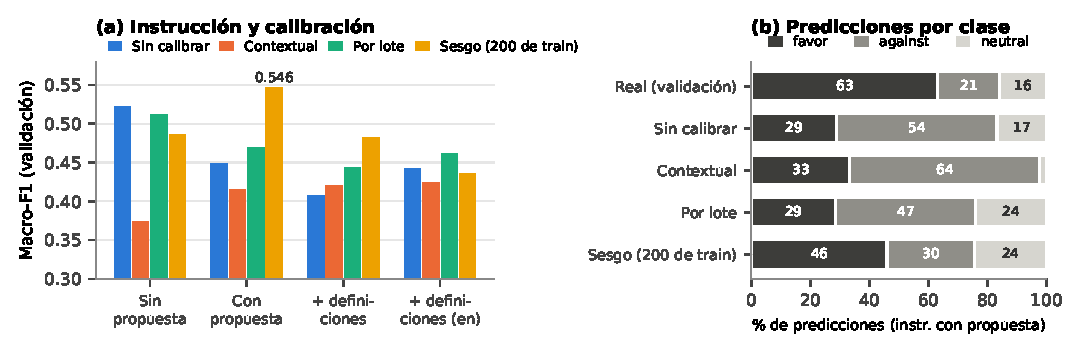
\includegraphics[width=0.95\textwidth]{figura_llm.pdf}
\caption{Zero-shot con Qwen2.5-1.5B (validación). (a) Macro-F1 según la instrucción y el método de calibración. (b) Distribución de las predicciones de la instrucción con la propuesta: sin calibrar predice \emph{against} de más; la calibración contextual elimina \emph{neutral}; el sesgo ajustado con 200 comentarios de train acerca la distribución a la real.}
\label{fig:llm}
\end{figure}

En test, el zero-shot calibrado obtiene \textbf{0,537} y el few-shot 0,530 $\pm$ 0,018 (sin calibrar: 0,474). Su ventaja está en \emph{neutral} (F1 0,40 contra 0,29 de BETO). El costo es la inferencia: $\approx$37\,s cada 1.000 comentarios en una T4 (372\,s con few-shot).

% =====================================================
\section{Evaluación comparativa}

\begin{table}[!htbp]
\centering
\resizebox{\textwidth}{!}{%
\begin{tabular}{lccccccccc}
\toprule
Modelo (test, $n=418$) & Macro-F1 & IC 95\% & Acc. & F1 fav. & F1 ag. & F1 neu. & Entren. & Inf. / 1.000 & Tamaño \\
\midrule
Referencia: siempre \emph{favor}      & 0,254 & -- & 0,615 & 0,761 & 0 & 0 & -- & -- & -- \\
Clásico: baseline TF-IDF + LogReg     & 0,309 & [0,27; 0,35] & 0,629 & 0,772 & 0,095 & 0,059 & 0,9\,s (CPU) & 0,08\,s (CPU) & 0,6\,MB \\
Clásico: n-gramas car.\ + LogReg bal. & 0,435 & [0,38; 0,49] & 0,529 & 0,667 & 0,346 & 0,292 & 3,6\,s (CPU) & 0,65\,s (CPU) & 1,3\,MB \\
Encoder: BETO congelado + LogReg      & 0,458 & [0,41; 0,51] & 0,502 & 0,604 & 0,459 & 0,311 & 7,6\,s (GPU) & 3,5\,s (GPU) & 439\,MB \\
Encoder: BETO fine-tuning (3 sem.)    & 0,495 $\pm$ 0,017 & [0,45; 0,54] & \textbf{0,611} & \textbf{0,731} & 0,464 & 0,290 & 72\,s (GPU) & 1,2\,s (GPU) & 439\,MB \\
LLM: Qwen zero-shot calibrado         & \textbf{0,537} & [0,48; 0,59] & 0,600 & 0,721 & \textbf{0,485} & \textbf{0,405} & 8\,s (calib.) & 37\,s (GPU) & 3,1\,GB \\
LLM: Qwen few-shot 12 (3 sel.)        & 0,530 $\pm$ 0,018 & [0,49; 0,58] & 0,600 & 0,716 & 0,481 & 0,392 & 75\,s (calib.) & 372\,s (GPU) & 3,1\,GB \\
\bottomrule
\end{tabular}}
\caption{Resultados en test. IC 95\% por \emph{bootstrap} (2.000 remuestreos del test). $\pm$ indica el desvío entre semillas o selecciones de ejemplos. El enfoque clásico se midió en CPU (2 núcleos de Colab) y el resto en una GPU T4. Los tiempos no incluyen la exploración de configuraciones ($\approx$3\,min de CPU para el clásico, $\approx$16\,min de GPU para BETO y $\approx$24\,min de GPU para el LLM).}
\label{tab:resultados}
\end{table}

\begin{figure}[!htbp]
\centering
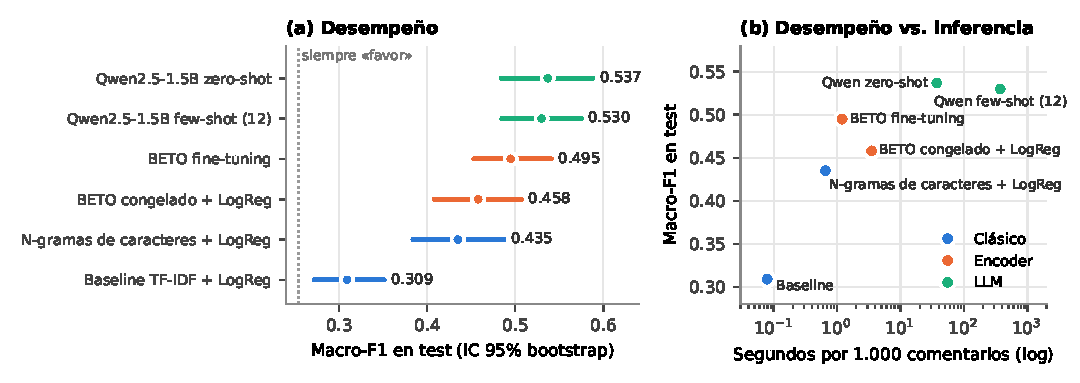
\includegraphics[width=0.95\textwidth]{figura_comparacion.pdf}
\caption{(a) Macro-F1 en test con IC 95\% por \emph{bootstrap}; la línea punteada es el clasificador que siempre predice \emph{favor}. (b) Macro-F1 contra el tiempo de inferencia cada 1.000 comentarios, en escala logarítmica.}
\label{fig:comparacion}
\end{figure}

\begin{figure}[!htbp]
\centering
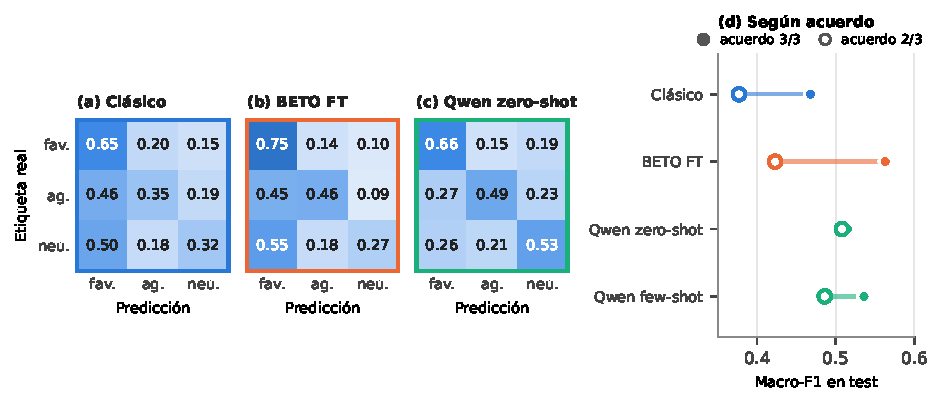
\includegraphics[width=0.95\textwidth]{figura_errores.pdf}
\caption{(a)--(c) Matrices de confusión en test del mejor modelo de cada enfoque, normalizadas por fila (BETO: promedio de 3 semillas). (d) Macro-F1 en test en los comentarios con acuerdo total (3/3) y parcial (2/3) entre anotadores.}
\label{fig:errores}
\end{figure}

\textbf{Desempeño.} El orden es LLM zero-shot (0,537) $>$ LLM few-shot (0,530) $>$ BETO fine-tuning (0,495) $>$ BETO congelado (0,458) $>$ clásico (0,435) (Tabla~\ref{tab:resultados}). Según el \emph{bootstrap} pareado, el LLM y BETO fine-tuning superan al clásico de forma significativa (+0,10 y +0,06). En cambio, la diferencia entre el LLM y BETO fine-tuning (+0,04, IC [$-$0,02; +0,10]) y la de few-shot contra zero-shot no son concluyentes. Ningún enfoque llega a 0,55. Las diferencias de costo, en cambio, son de varios órdenes de magnitud (Fig.~\ref{fig:comparacion}b): el LLM es $\approx$30 veces más lento que BETO en la misma GPU y $\approx$60 veces más lento que el clásico en CPU, y pesa unas 2.300 veces más que el modelo clásico.

\textbf{Dónde gana cada uno.} Las matrices de confusión (Fig.~\ref{fig:errores}a--c) muestran a dónde van los errores. El modelo clásico y BETO mandan la mitad de los \emph{neutral} a \emph{favor} (BETO recupera solo el 27\% de los \emph{neutral}), mientras que el LLM recupera el 53\%. Los tres mandan entre el 27\% y el 46\% de los \emph{against} a \emph{favor}. BETO fine-tuning es el mejor en los comentarios con acuerdo total entre anotadores (Macro-F1 0,563), pero cae 0,14 en los de acuerdo parcial. El LLM casi no cae (0,515 $\rightarrow$ 0,508; Fig.~\ref{fig:errores}d): es el más robusto ante la ambigüedad, y de ahí viene su ventaja en \emph{neutral}. Además, los enfoques se equivocan en comentarios distintos ($\kappa$ de Cohen entre sus predicciones de 0,2 a 0,35): combinándolos perfectamente se acertaría el 90\% del test, lo que sugiere que un ensamble podría mejorar los resultados. A la vez, el 10\% de los comentarios no lo acierta ningún modelo, y el 77\% de ellos tiene acuerdo parcial entre anotadores. Los errores típicos son críticas que en realidad apoyan la propuesta (una crítica dura a una concejala es \emph{favor} de su reprobación) y apoyos implícitos que dependen de entender la propuesta.

% =====================================================
\section{Conclusiones}

\textbf{¿Cuándo conviene cada enfoque?} En esta tarea, la complejidad del modelo trajo mejoras reales pero moderadas (+6 a +10 puntos de Macro-F1 sobre el clásico), a cambio de costos de cómputo de dos a tres órdenes de magnitud mayores. Además, decisiones ``baratas'' tuvieron tanto impacto como cambiar de modelo: balancear las clases sumó 15 puntos al modelo clásico, y calibrar el LLM con 200 ejemplos sumó 10 en validación.
\begin{itemize}
  \item \textbf{ML clásico} cuando el volumen es muy grande, no hay GPU o se necesita interpretabilidad. Con balanceo de clases es una línea de base obligatoria: entrena en segundos, clasifica un millón de comentarios en $\approx$11\,min en CPU y pesa 1\,MB. Su límite es estructural: no puede modelar la relación entre el comentario y la propuesta.
  \item \textbf{Encoder con fine-tuning} cuando hay datos etiquetados ($\approx$2.000 alcanzaron) y una GPU para entrenar, y el modelo se va a usar sobre muchos datos: rinde cerca del LLM con una inferencia $\approx$30 veces más barata. Usado congelado, en cambio, no se justifica, porque cuesta casi lo mismo y mejora poco.
  \item \textbf{LLM con prompting} cuando hay pocos datos etiquetados, se necesita un prototipo rápido o la tarea cambia seguido, y el volumen es moderado ($\approx$10\,h por millón de comentarios en una T4). Conviene usarlo en zero-shot y calibrado: sin calibrar rinde por debajo de BETO, y el few-shot multiplicó el costo sin mejorar. No es estrictamente ``sin datos'': necesita un conjunto chico de ejemplos etiquetados para calibrar.
\end{itemize}

\textbf{Limitaciones.} El test es chico (IC de $\approx\pm$0,05). Evaluamos un solo LLM, y además chico (un modelo de 7B probablemente aprovecharía mejor la propuesta y los ejemplos). Excluimos los comentarios sin mayoría, y \emph{neutral} sigue siendo la clase más difícil para todos los enfoques.

\textbf{Reflexión grupal.} Este trabajo nos permitió entender que no existe un modelo que sea siempre la mejor opción, sino que la elección depende del problema, los datos disponibles y los recursos con los que se cuenta. También vimos que un mayor nivel de complejidad no garantiza mejores resultados y que decisiones como el balanceo de clases o la calibración pueden tener tanto impacto como la elección del modelo. Nos llevamos la importancia de evaluar no solo el desempeño, sino también los costos y las limitaciones de cada enfoque para elegir una solución que sea realmente viable.

\end{document}
